%POLAR COORDINATES
%The print template for A4 paper (portrait)
%Author: Zoran Nikolic
\documentclass[12pt]{article}
\usepackage[margin=0.5in,paper=a4paper]{geometry} %Shrinking margins to 0.5in
\usepackage[x11names,rgb]{xcolor}                     %Additional colors
\usepackage{tikz}
\usepackage{euler}                                %Nicer numbers


%Note about the colors: 
%  The color of the "ray" lines should not be
%  black or gray as on some printers, significant
%  aliasing distorsion becomes visible.

\begin{document}
\thispagestyle{empty} %Please, no page numbers or similar

\begin{center}
  \begin{tikzpicture}

% draw the sections
\foreach \t [evaluate = \t as \tfrac using \t/8] in {0,...,7}
{
  % to rotate through the colors
  \definecolor{fillc}{hsb}{\tfrac,.5,1}
  % to draw the slices
  %\draw [fill=fillc] (0,0) -- ({1.40625*2^\t}:{8-\t}) arc ({1.40625*2^\t}:{1.40625*2^(\t+1)}:{8-\t}) -- cycle;
  \draw [fill=fillc] (0,0) -- ({1.40625*2^\t}:6) arc ({1.40625*2^\t}:{1.40625*2^(\t+1)}:6) -- cycle;
}
% draw radials for subnet breaks
\foreach \t in {2^0,2^...,2^8}
  \draw [draw=red, thick] (0,0) -- ({\t*1.40625}:8);
  
%Circles 
\foreach \r in {1, 2,...,7}
  \draw[SteelBlue3] (0,0) circle (\r);    
%      \foreach \r in {0.5, 1.5,...,7}
%        \draw[Azure4, thin] (0,0) circle (\r);

%angle marks
\foreach \a in {0, 2,...,255}
  \draw[Azure4] (\a*1.40625:7) -- (\a*1.40625:8);
\foreach \a in {0, 4,...,255}
  \draw[Azure4] (\a*1.40625:6) -- (\a*1.40625:7);
\foreach \a in {0, 8,...,255}
  \draw[Azure4] (\a*1.40625:4) -- (\a*1.40625:6);      
\foreach \a in {0, 16,...,255}
  \draw[Azure4] (\a*1.40625:2) -- (\a*1.40625:4); 
\foreach \a in {0, 32,...,255}
  \draw[Azure4] (0, 0) -- (\a*1.40625:8);


%    %Main rays
    \foreach \a in {0, 90,...,359}
      \draw[very thick] (0, 0) -- (\a:8);


%    %Radius labels (background filled white)
    \foreach \r [evaluate = \r as \n using 30-\r] in {0,...,7}
    \draw ({1.40625*2^\r}:10) node[inner sep=1pt,below=3pt,rectangle,fill=white] {$\n$};

% Angle labels  
%    \foreach \a in {0, 15,...,359}
%      \draw (\a: 10) node {$\a^\circ$};
\foreach \a in {0, 4,...,255}
	\draw (\a*1.40625 : 8.5) node {$\a$};

%\foreach \a [evaluate = \a as \aa using (32-ceil(log2(\a))] in {1, 1,...,31}
%\foreach \a [evaluate = \a as \aa using (2^\a)] in {1, 1,...,8}
%	\draw ( {\aa*1.40625} : 9.5 ) node {\pgfmathparse{32-\a}$\pgfmathresult$};

%\filldraw[fill=green!20!white, draw=green!50!black]
%	(0,0) -- (8,0) arc (8,8) -- (0,0);
%	(0:0) -- (0:8.5) arc ( 4 : 8.5 ) -- (0:0);

%\filldraw[fill=green!20!white, draw=green!50!black]
%	(0,0) -- (7,0) arc (0:{4*1.40625}:7) -- cycle;


%\filldraw[fill=red!20!white, draw=green!50!black]
%	(0,0) -- ({0*1.40625}:7) arc (0:{4*1.40625}:7) -- cycle;
%\filldraw[fill=red!20!white, draw=green!50!black]
%	(0,0) -- ({4*1.40625}:7) arc (0:{8*1.40625}:7) -- cycle;
%\filldraw[fill=red!20!white, draw=green!50!black]
%	(0,0) -- ({8*1.40625}:7) arc ({16*1.40625}:7) -- cycle;
%\foreach \t [evaluate = \t as \p using 2^\t] in {0, 1,...,8} 
%	\draw [draw=red] (0,0) -- (\t:6) arc (\t:\p:6) -- cycle;



%Central point
    \draw[fill=red] (0,0) circle(0.7mm);
  \end{tikzpicture}
\end{center}



\end{document}
